%%%%%%%%%%%%%%%%%%%%%%%%%%%%%%%%%%%%%%%%%
% University/School Laboratory Report
% LaTeX Template
% Version 3.1 (25/3/14)
%
% This template has been downloaded from:
% http://www.LaTeXTemplates.com
%
% Original author:
% Linux and Unix Users Group at Virginia Tech Wiki 
% (https://vtluug.org/wiki/Example_LaTeX_chem_lab_report)
%
% License:
% CC BY-NC-SA 3.0 (http://creativecommons.org/licenses/by-nc-sa/3.0/)
%
%%%%%%%%%%%%%%%%%%%%%%%%%%%%%%%%%%%%%%%%%

%----------------------------------------------------------------------------------------
%	PACKAGES AND DOCUMENT CONFIGURATIONS
%----------------------------------------------------------------------------------------

\documentclass{article}

\usepackage[version=3]{mhchem} % Package for chemical equation typesetting
\usepackage{siunitx} % Provides the \SI{}{} and \si{} command for typesetting SI units
\usepackage{graphicx} % Required for the inclusion of images
\usepackage{natbib} % Required to change bibliography style to APA
\usepackage{amsmath} % Required for some math elements 

\setlength\parindent{0pt} % Removes all indentation from paragraphs

\usepackage{hyperref} % For hyperlinks
\hypersetup{
    colorlinks=true,
    linkcolor=blue,
    filecolor=magenta,      
    urlcolor=black,
}


\usepackage{ragged2e} % For alignment

\renewcommand{\labelenumi}{\alph{enumi}.} % Make numbering in the enumerate environment by letter rather than number (e.g. section 6)

%\usepackage{times} % Uncomment to use the Times New Roman font

%----------------------------------------------------------------------------------------
%	DOCUMENT INFORMATION
%----------------------------------------------------------------------------------------

\title{Inferential Modeling and Visualization of the COVID-19 Outbreak in Ontario \\ 
		\large A Proposal to integrate the Open Database of Healthcare Facilities and Proximity Data with COVID-19 Data}


\author{Shreeram \textsc{Murali} \\ KT \textsc{Hobbs} \\ Ngan \textsc{Lyle} \\ Sofia \textsc{Bahmutsky}}

\date{\today} % Date for the report

\begin{document}

\maketitle % Insert the title, author and date

\begin{center}
\begin{tabular}{l r}
Partners: & Bruno St-Aubin \\ % Partner names
& Marian Radulescu \\
Instructor: & Scott Fazackerley % Instructor/supervisor
\end{tabular}
\end{center}

% If you wish to include an abstract, uncomment the lines below
% \begin{abstract}
% Abstract text
% \end{abstract}

%----------------------------------------------------------------------------------------
%	SECTION 1
%----------------------------------------------------------------------------------------

\section{Introduction}
Since its initial appearance in China on December 31, 2019, Coronavirus disease, or COVID-19, has evolved to a global pandemic --- a novel disease to which there is little pre-existing immunity, that becomes epidemic in many countries. At the time of writing, COVID-19 has spread to more than 180 countries (1). Worldwide there are greater than 3 million confirmed cases and greater than 230,000 deaths (2). In Canada, there have been almost 60,000 confirmed cases and in Ontario alone, there have been more than 19,000 cases and 1,400 deaths (3). Therefore, this proposal seeks to integrate a number of open source databases to provide insight into the COVID-19 outbreak in Ontario. 

Specifically, we have two primary focusses; first, it has become clear that seniors shoulder a disproportionate burden of disease. In fact, almost half of fatalities in Canada are related to outbreaks among seniors in long term care (LTC) homes (4). Moreover, we aim to explore the spread of COVID-19 among LTC homes in Canada. Second, different Ontario public health unit (PHU) regions have experienced different levels of disease activity. This may be related to characteristics of individual regions, such as proximity to amenities; therefore, we will also explore the relationship between various measures of proximity and COVID-19 disease rates. 


% If you have more than one objective, uncomment the below:
%\begin{description}
%\item[First Objective] \hfill \\
%Objective 1 text
%\item[Second Objective] \hfill \\
%Objective 2 text
%\end{description}

\section{Data Sources}

The following open data sources will be used:

\begin{description}

\item[Open Database for Health Facilities (ODHF) data]
A comma-separated file of health facility information across Canada with missing address information.

\item[Confirmed Positive Cases of COVID-19 in Ontario (5)]
A comma-separated file of confirmed cases and deaths in Ontario.

\item[Health Region level COVID Data(6)]
A feature server from Statistics Canada.

\item[Proximity data for transit, health care, and/or pharmacies]
A comma-separated file of proximity metrics across Canada on the regional level. We will focus on data for Ontario.

\end{description} 

In addition, COVID-19 statistics for LTC homes in Ontario will be scraped from open Ontario websites (7, 8).

  
%----------------------------------------------------------------------------------------
%	SECTION 2
%----------------------------------------------------------------------------------------

\section{Objectives}

There are two main objectives:

\begin{center}
\begin{itemize}
\item To produce an inferential statistical model of factors that may contribute to COVID-19 outbreaks in LTC homes in Ontario. 

\item To produce an inferential statistical model of factors that may contribute to COVID-19 outbreaks at the level of PHU regions in Ontario.
\end{itemize}
\end{center}


\section{Methods}
\subsection{Data Preparation}

For objective one, we will first create a database of LTC homes in Ontario. Data will be drawn from the ODHF and web scraping of open Ontario websites. This database of LTC homes will include facility name, address, geolocation data, number of beds, facility size, home type (e.g. public or private), short stay status, as well as number and type (e.g. complaints or critical incidents) of inspection reports. In addition COVID-19 statistics for each LTC home will be webscraped from a Government of Ontario website including numbers of resident infections, resident deaths and staff infections. This COVID-19 data will then be merged with the LTC homes database. 

For objective two, proximity data, which is currently available at the level of dissemination blocks, will be aggregated at the PHU region level. These data can then be merged with open COVID-19 data for Ontario for analysis. 


\subsection{Statistical Analysis}
We will implement principle component analysis (PCA) regression, an unsupervised statistical method to determine the factors that are most influential in explaining the variation between LTC homes and PHUs. For objective one (involving the LTC homes), we will also be implementing factor analysis (FA). FA gives us the ability to assess for latent explanatory variables which may be important because variation between LTC homes may be driven by factors that are not explicitly included in our LTC homes database. 

\subsection{Visualization}
Once the statistical analysis is complete, interactive maps will be created that depict location and severity of COVID-19 cases among LTC homes in Ontario. Influential factors reported by PCA and FA analyses will be incorporated as metadata. This will be accomplished using the shape files from the ODB as well as GIS, and D3. 


\section{Deliverables}
\begin{center}
\begin{itemize}
\item A database of LTC homes in Ontario.

\item A method to aggregate proximity data to the PHU region level.

\item Inferential models, which will assess the importance of predictor variables in relation to the COVID-19 outbreaks in LTC homes and in different Ontario PHU regions.

\item Visualizations integrating LTC homes, proximity metrics and COVID-19 outbreak data in Ontario. 

\item A report including exploratory analyses of patterns and/or connections between the LTC homes data, the proximity data, and the COVID-19 data.

\end{itemize}
\end{center}

\subsection{Schedule}

\begin{figure}[h]
\begin{center}
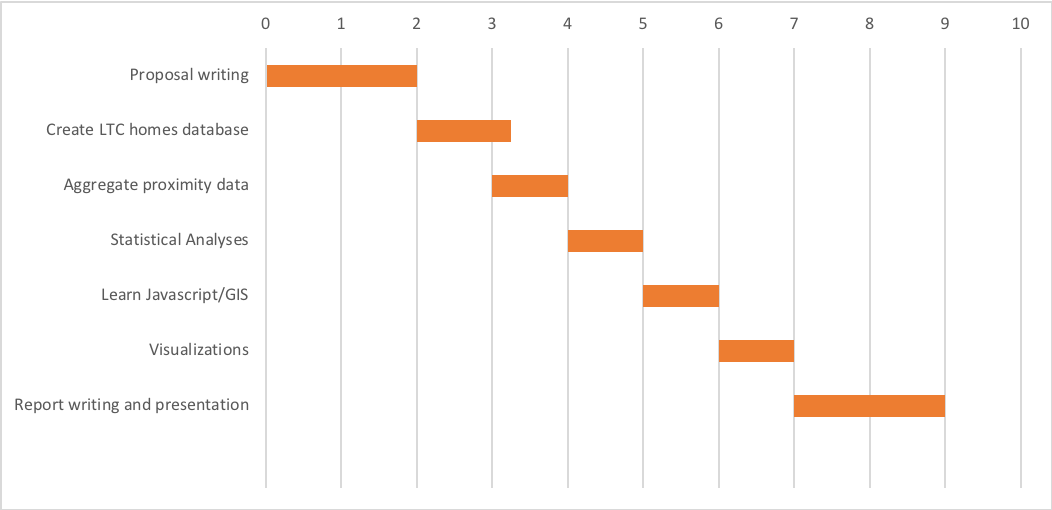
\includegraphics[width=0.65\textwidth]{schedule} % Include the image placeholder.png
\caption{Schedule for completion of tasks for the project in weeks.}
\end{center}
\end{figure}

\subsubsection{Schedule Details}
\begin{table}[h!]
	\begin{center}
   	 \caption{Details for Selected Tasks}
   	 \label{tab:table1}
		\begin{tabular}{p{35mm}|p{75mm}|p{20mm}}
			\textbf{Task} & \textbf{Details} & \textbf{Tools}\\
 			\hline\hline
 			Create LTC homes database & \textbf{1.} Using the ODHF and web scraping, create a database of LTC homes in Ontario \newline \textbf{2.} Merge scraped data & python \\
 			\hline
 			Aggregating proximity data & Aggregate proximity data from dissemination block level to PHU levels & python, R\\
 			\hline
			Statistical Analyses & PCA and FA & R\\
			\hline
			Learn Javascript/GIS & Learn how to implement using D3 & python, R\\
			\hline
			Visualizations & \textbf{1.} Interactive chloropleth map of LTC homes in Ontario with COVID-19 status and metadata \newline \textbf{2.} Interactive choropleth map of COVID-19 case numbers and proximity measures by PHU region in Ontario & R, arcGIS, D3, Mapbox\\

		\end{tabular}

	\end{center}
\end{table}



The project will begin as soon as permission is granted to proceed and will proceed according to the schedule shown in \textbf{Figure 1}. Details for selected tasks are shown in \textbf{Table 1}. The final report will be completed by the week of June 15th.


\section{Limitations}

The proposed project, including data preparation, analysis, visualization and report writing, is being undertaken on a compressed timeline and includes exposure to new tools and programming languages such as JavaScript and GIS. As a result, the deliverables will likely require assistance and further review before they are publishable.
 
\section{Conclusion}
This project aligns with Statistics Canada’s aims to produce high quality accessible visualization and analysis products that showcase usability of open data in complex analytical cases.



%----------------------------------------------------------------------------------------
%	BIBLIOGRAPHY
%----------------------------------------------------------------------------------------


\section{Bibliography}

\textbf{1} Dong, E., Du, H., \& Gardner, L. (2020). An interactive web-based dashboard to track COVID-19 in real time. Lancet Infect Dis. \href{ https://doi.org/10.1016/S1473-3099(20)30120-1}{ https://doi.org/10.1016/S1473-3099(20)30120-1}.\\

\\
\textbf{2} World Health Organization. (2020, March 3). Coronavirus disease 2019 (COVID-19) Situation Report --- 42. Retrieved from \href{https://www.who.int/docs/default-source/coronaviruse/situation-reports/20200503-covid-19-sitrep-104.pdf?sfvrsn=53328f46_4}{https://www.who.int/docs/default-source/coronaviruse/situation-reports/20200503-covid-19-sitrep-104.pdf?sfvrsn=53328f46\_4}\\

\textbf{3} Government of Ontario. (2020). How Ontario is responding to COVID-19. Retrieved from \href{https://www.ontario.ca/page/how-ontario-is-responding-covid-19}{https://www.ontario.ca/page/how-ontario-is-responding-covid-19}.\\

\textbf{4} Weeks, C., Mahoney, J., Stone, L., \& Ha, T.T. (2020, April 13). Outbreaks at seniors’ homes linked to almost half of COVID-19 deaths in Canada, Theresa Tam says. The Globe and Mail. Retrieved from \href{https://www.theglobeandmail.com/canada/article-outbreaks-at-seniors-homes-linked-to-almost-half-of-covid-19-deaths/}{https://www.theglobeandmail.com/canada/article-outbreaks-at-seniors-homes-linked-to-almost-half-of-covid-19-deaths/} \\

\textbf{5} Government of Ontario. (2020). Confirmed positive cases of COVID19 in Ontario. Retrieved from \href{https://data.ontario.ca/dataset/confirmed-positive-cases-of-covid-19-in-ontario/resource/455fd63b-603d-4608-8216-7d8647f43350}{https://data.ontario.ca/dataset/confirmed-positive-cases-of-covid-19-in-ontario/resource/455fd63b-603d-4608-8216-7d8647f43350}.\\

\textbf{6} Statistics Canada. (2020). ArcGIS REST Services Directory. Retrieved from \href{https://services1.arcgis.com/HsjBaDykC1mjhXz9/arcgis/rest/services/covid_19_by_health_regions_pro_view/FeatureServer}{https://services1.arcgis.com/HsjBaDykC1mjhXz9/arcgis/rest/services/covid\_19\_by\_health\_regions\_pro\_view/FeatureServer}.\\

\textbf{7} Government of Ontario. (2020). How Ontario is responding to COVID-19. \href{https://www.ontario.ca/page/how-ontario-is-responding-covid-19}{https://www.ontario.ca/page/how-ontario-is-responding-covid-19}.\\

\textbf{8} Public Reporting for Long-Term Care. Retrieved from \href{http://publicreporting.ltchomes.net/en-ca/LHIN_Map.aspx}{http://publicreporting.ltchomes.net/en-ca/LHIN_Map.aspx}. \\



%----------------------------------------------------------------------------------------


\end{document}